\documentclass[../main.tex]{subfiles}

\begin{document}
\begin{problema}
	El estado de tensión a través de un medio continuo está dado respecto
	a los ejes cartesianos por el siguiente tensor de esfuerzos:

	\begin{equation*}
		\sigma_{ij} =
		\begin{pNiceMatrix}
			3x_{1}     & 5x_{2}^{2} & 0      \\
			5x_{2}^{2} & 0          & 2x_{3} \\
			0          & 2x_{3}     & 0      \\
		\end{pNiceMatrix}
	\end{equation*}

	Usando coordenadas cilíndricas determinar lo siguiente:

	\begin{enumerate}
		\item El vector de esfuerzo que actúa en el punto \(\boldvect\vect{P}(2, 1, \sqrt{3})\) de
		      un plano que es tangente en \(\boldvect\vect{P}\) a la superficie cilíndrica
		      \(x_{2}^{2} + x_{3}^{3} = 4\). La figura muestra el esquema de la superficie
		      cilíndrica.
		\item La componente perpendicular al plano, es decir, el esfuerzo normal.
		\item La componente tangencial al plano, es decir, el esfuerzo tangente.
	\end{enumerate}

	\begin{figure}[htb]
		\centering
		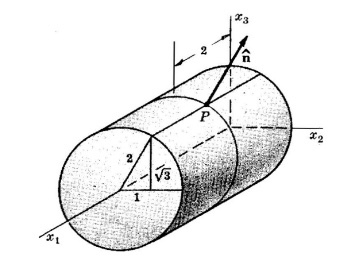
\includegraphics[width=.45\textwidth]{figs/problema02-001.jpg}
	\end{figure}
\end{problema}
\end{document}
